% Diese Zeile bitte -nicht- aendern.
\documentclass[course=erap]{aspdoc}

%%%%%%%%%%%%%%%%%%%%%%%%%%%%%%%%%
%% TODO: Ersetzen Sie in den folgenden Zeilen die entsprechenden -Texte-
%% mit den richtigen Werten.
\newcommand{\theGroup}{288} % Beispiel: 42
\newcommand{\theNumber}{A500} % Beispiel: A123
\author{Miguel Ryan \and Ryan Kafoor \and Welsen Evan Efendi}
\date{Sommersemester 2023} % Beispiel: Wintersemester 2019/20
%%%%%%%%%%%%%%%%%%%%%%%%%%%%%%%%%

% Diese Zeile bitte -nicht- aendern.
\title{Gruppe \theGroup{} -- Abgabe zu Aufgabe \theNumber}


\usepackage{amsmath}
\usepackage{amssymb}
\usepackage{xcolor}
\usepackage{fancyvrb}
\usepackage{diagbox}
\usepackage{graphicx}
\usepackage{upgreek} %for \upmu: microseconds
\usepackage{svg}


\begin{document}
\maketitle
\section{Einleitung}
Internet ist heutzutage ein Bestandteil unseres alltäglichen Lebens geworden. 
Wenn wir Websites besuchen, online shoppen, oder auch sich mit unseren Freunden via soziale Medien austauschen, findet Fluss von Daten statt. Oft sind uns diese Daten -wie unsere Bankinformationen, Kommunikationsinhalte von größer Bedeutung. Da kommt die Verschlüsselung zum Einsatz, um die Sicherheit unserer Daten zu gewährleisten.


Bei der symmetrischen Verschlüsselung, die mit einem geheimen Schlüssel sowohl zum Codieren als 
auch zum Decodieren arbeitet, gibt es zwei Chiffrearten, die Strom- und Blockchiffre. 
Eine Stromchiffre verschlüsselt eine beliebig lange und fortlaufende Klartextnachricht Bit 
für Bit oder Byte für Byte. Genauer wird jedes Bit oder Byte des Klartextes mit einem Bit bzw. 
Byte eines Schlüsselstroms durch die logische XOR-Operation verknüpft. Daher ist die 
Stromchiffre besonders für Echtzeit-Verschlüsselung oder große Menge an Daten geeignet. Zur 
Veranschaulichung der Funktionsweise einer Stromchiffre haben wir ein Beispiel dargestellt: 

\begin{center}
Klartext: HELLO

Schlüssel: ABCDE
\end{center}

Als Binärstrings:

\begin{center}
Klartext: 01001000 01000101 01001100 01001100 01001111

Schlüssel: 01000001 01000010 01000011 01000100 01000101
\end{center}

Um den Klartext zu verschlüsseln, generieren wir einen Schlüsselstrom gleicher Länge zum Klartext 
durch ein arbiträres Verschlüsselungsverfahren. Beispielsweise hätten wir einen Schlüsselstrom wie 
folgt:

\begin{center}
Schlüsselstrom: 01111001 01101111 01011010 01110111 01110111
\end{center}

Da wir den Schlüsselstrom schon haben, führen wir den bitweisen XOR-Operator zwischen jedem Bit 
unseres Klartextes und unseres Schlüsselstroms durch und erhalten den Chiffretext:

\begin{center}
Chiffretext: 00110001 00101010 00010110 00111011 00111000
\end{center}

Durch erneute Anwendung des bitweisen XOR-Operators auf den Chiffretext und denselben Schlüsselstrom kann der 
verschlüsselte Text wieder entschlüsselt werden. Für ein besseres Verständnis haben wir ein Beispiel dafür:
\begin{center}
\begin{tabular}{c}
Klartext\\
\\
Schlüsselstrom\\
\\
Chiffretext\\
\end{tabular}
\quad
\begin{tabular}{|c|}
\hline
01001000\\
\hline
\(\oplus\) \\
\hline
01111001 \\
\hline
= \\
\hline
01001000 \\
\hline
\end{tabular}
\quad
\begin{tabular}{c}
Chiffretext\\
\\
Schlüsselstrom\\
\\
Klartext\\
\end{tabular}
\quad
\begin{tabular}{|c|}
\hline
01001000\\
\hline
\(\oplus\) \\
\hline
01111001 \\
\hline
= \\
\hline
01001000\\
\hline
\end{tabular}
\end{center}

In dieser Ausarbeitung werden wir uns mit einer von Daniel J. Bernstein erfundenen 
Stromchiffre, nämlich mit der Salsa20/20 beschäftigen \cite{bernstein2005salsa20}. Das Salsa20/20 nimmt einen 256-Bit-Key (32 Byte), eine 64-Bit-Nonce 
(8 Byte) und einen 64-Bit-Block-Counter und erzeugt daraus in insgesamt 20 Runden einen 
512-Bit-Block-Keystream. Intern wird eine \(4 \times 4\)-Matrix aus 16 32-Bit vorzeichenlosen 
Little-Endian-Ganzzahlen gebildet und der Anfangszustand dieser Matrix \(S\) ist gegeben durch: 
\vspace{0.5cm}
\begin{center}
\begin{math}
    \begin{pmatrix}
    0$x$61707865 & K_0 & K_1 & K_2\\
    K_3 & 0$x$3320646e & N_0 & N_1\\
    C_0 & C_1 & 0$x$79622d32 & K_4\\
    K_5 & K_6 & K_7 & 0$x$6b206574\\
    \end{pmatrix}
\end{math}
\end{center}
\vspace{0.5cm}

%cite source for nothing up my sleeve number
Die 4 Konstanten auf der Diagonalen entsprechen “\textit{expa}”, ”\textit{nd 3}”, ”\textit{2-by}”, ”\textit{te k}” in ASCII (“\textit{expand 32-byte k}”). Diese sind pseudozufällige Konstante, die einen Zweck hat, dem Verdacht entgegenzuwirken, dass eine “Hintertür” dadurch eingebaut wird, durch die das ganze Verfahren exploitieren kann. Deswegen heißen die in einem kryptografischen Verfahren “Nothing-up-my-sleeve Number”. \(K_i\) steht für den \(i\)-ten Teil des Schlüssels (\(K_0\) steht also für die ersten 4 Bytes in Little-Endian-Reihenfolge des Schlüssels, \(K_1\) für die zweiten 4 bytes usw.). Analog gilt für Nonce \(N_i\) und Counter \(C_i\). Der Counter hier ist im Gegensatz zu Nonce und Key keine Eingabe dieses Algorithmus, weil er am Anfang mit dem Wert \(0\) initialisiert und nach jedem Keystream-Block inkrementiert wird.
%should nonce be explained?
Die Erstellung des Keystream-Blocks dieses Verfahrens erfolgt über die 20 Runden des sogenannten \textit{Add-Rotate-XOR} (kurz ARX)- Schemas. Im Folgenden wird der Ablauf einer Runde dargestellt.

Um ein besseres Verständnis zu haben, definieren wir einige Operatoren wie folgt:

\begin{enumerate}
    \item \(x \lll y\) bezeichne die Linksrotation von \(x\) um \(y\) Bit.
    \item \(x \ggg y\) bezeichne die Rechtsrotation von \(x\) um \(y\) Bit.
    \item \(\oplus\) bezeichne den binären XOR-Operator.
\end{enumerate}

Wir verwenden die übliche Schreibweise $a_{i,j} \in A$ um einen einzelnen Eintrag der obigen Matrix anzugeben. Jedes Wort unter der Diagonalen wird dann wie folgt modifiziert:
\begin{align*}
a_{2,1} &= ((a_{1,1} + a_{4,1}) \lll 7) \oplus a_{2,1} \\
a_{3,2} &= ((a_{2,2} + a_{1,2}) \lll 7) \oplus a_{3,2} \\
a_{4,3} &= ((a_{3,3} + a_{2,3}) \lll 7) \oplus a_{4,3} \\
a_{1,4} &= ((a_{4,4} + a_{3,4}) \lll 7) \oplus a_{1,4}
\end{align*}
%
% For better readability
%
Analog zur obigen Darstellung modifizieren wir die Einträge aber diesmal wird um 9 Bit rotiert:
\begin{align*}
a_{3,1} &= ((a_{1,1} + a_{2,1}) \lll 9) \oplus a_{3,1} \\
a_{4,2} &= ((a_{2,2} + a_{3,2}) \lll 9) \oplus a_{4,2} \\
a_{1,3} &= ((a_{3,3} + a_{4,3}) \lll 9) \oplus a_{1,3} \\
a_{2,4} &= ((a_{4,4} + a_{1,4}) \lll 9) \oplus a_{2,4}
\end{align*}
%
% For better readability
%
Dasselbe passiert nun eine Zeile nach unten versetzt. Nun wird um 13 Bit rotiert:
\begin{align*}
a_{4,1} &= ((a_{3,1} + a_{2,1}) \lll 13) \oplus a_{4,1} \\
a_{1,2} &= ((a_{4,2} + a_{3,2}) \lll 13) \oplus a_{1,2} \\
a_{2,3} &= ((a_{1,3} + a_{4,3}) \lll 13) \oplus a_{2,3} \\
a_{3,4} &= ((a_{2,4} + a_{1,4}) \lll 13) \oplus a_{3,4}
\end{align*}
%
% For better readability
%
Letztlich modifizieren wir die Diagonale wie folgt: 
\begin{align*}
a_{1,1} &= ((a_{4,1} + a_{3,1}) \lll 18) \oplus a_{1,1} \\
a_{2,2} &= ((a_{1,2} + a_{4,2}) \lll 18) \oplus a_{2,2} \\
a_{3,3} &= ((a_{2,3} + a_{1,3}) \lll 18) \oplus a_{3,3} \\
a_{4,4} &= ((a_{3,4} + a_{2,4}) \lll 18) \oplus a_{4,4}
\end{align*}
%
% For better readability
%
Das finale Ergebnis einer Runde entsteht, indem die Matrix \(A\) transponiert wird:

\begin{center}
	\(A = A^T\)
\end{center}
Am Ende aller Runden wird die aktuelle Matrix \(A\) noch auf den Startzustand \(S\) addiert.
Somit ergibt sich für den 64-Byte-Ausgabeblock \(O\):
%was einer Runde

\begin{center}
	\(O = A + S\)
\end{center}
Alle Additionen werden auf dem Restklassenring \(Z/(32)\) durchgeführt.

Wie bereits erwähnt, dieselbe Funktion kann beim Verschlüsseln und Entschlüsseln verwendet werden. Um die verschlüsselte Nachricht richtig zu entschlüsseln, müssen derselbe Key und dieselbe Nonce eingegeben werden. Außerdem gilt dabei die verschlüsselte Nachricht als Eingabe.



Für einen bestimmten Key und eine bestimmte Nonce könnte die Salsa20/20-Funktion \(2^{64}\) * \(2^{6}\) = \(2^{70}\) Zeichen oder Bytes ver- oder entschlüsseln. Grund dafür ist, dass der maximale Counter-Wert \(2^{64}-1\) ist und für jeden Counter-Wert ein 64-Byte-Keystream-Block (\(2^{6}\)) erzeugt werden kann.

Im Folgenden beschreiben wir den Lösungsansatz, den wir für dieses Programm gewählt haben, wie korrekt das Programm ist, und analysieren auch seine Leistung. 





\section{Lösungsansatz}
Dieser Abschnitt beschreibt die grundlegenden Komponenten und ihre Funktionen des gesamten C Programms sowie den Ansatz, den wir zur Implementierung des Salsa20-Verschlüsselungsalgorithmus und zur Optimierung gewählt haben. Wir werden auch andere mögliche Optimierungsideen abdecken, die wir in der endgültigen Implementierung nicht verwendet haben, und begründen, warum wir uns gegen die Verwendung solcher Ideen entschieden haben.

Die Hauptberechnung des Algorithmus ist in zwei Hauptfunktionen unterteilt. 
\begin{enumerate}
    \item Eine Kernfunktion, die eine 4x4-Matrix mit einem bestimmten Zählwert, Key und Nonce berechnet. Diese Funktion hat die Signatur
    \begin{Verbatim}[commandchars=\\\{\}]
    \textcolor{blue}{void} salsa20_core(\textcolor{blue}{uint32_t} output[16], \textcolor{blue}{const uint32_t} input[16])
    \end{Verbatim}
    Dabei wird die Eingabematrix, wie im Algorithmus beschrieben, entsprechend dem Anfangszustand initialisiert. Das Ergebnis der Funktion wird in der Ausgangsmatrix zurückgegeben.
    \item Eine Verschlüsselungsfunktion, die die XOR-Operation für jedes Byte des Klartextes mit dem entsprechenden Byte aus der Ausgabematrix der Kernfunktion ausführt.
    \begin{Verbatim}[commandchars=\\\{\}]
    \textcolor{blue}{void} salsa20_crypt(\textcolor{blue}{size_t} mlen, \textcolor{blue}{const uint8_t} msg[mlen], \textcolor{blue}{uint8_t}
    cipher[mlen], \textcolor{blue}{uint32_t} key[8], \textcolor{blue}{uint64_t} iv)
    \end{Verbatim}
\end{enumerate}


\subsection{Naiver Ansatz}
Es wurde ein sehr naiver Ansatz ohne jegliche Optimierungen gewählt, der in der Vergleichsimplementierung neben der Haupt- oder optimierten Implementierung implementiert wird, damit er als Referenz zur Vergleichung der Leistungssteigerung in der optimierten Version des Verschlüsselungsalgorithmus verwendet werden kann. 
\subsubsection{Verschlüsselungsfunktion}
In der naiven Implementierung der Verschlüsselungsfunktion \verb {salsa20_crypt_v1{ wird der Klartext in Blöcke von 64 Bytes aufgeteilt und verarbeitet, da der Keystream-Block in Form einer 4x4-Matrix mit 4-Byte-Elementen mit einer Gesamtgröße von 64 Byte erzeugt wird. Dieser Keystream-Block wird dann verwendet, um die XOR-Operation mit jedem einzelnen Byte des Klartextblocks auszuführen und das Ergebnis an der entsprechenden Position in \verb{cipher{ zu speichern. Für den nächsten Block von dem Klartext wird derselbe Vorgang ausgeführt, mit dem einzigen Unterschied, dass der Counter beim Erzeugen des nächsten Keystream-Blocks um eins erhöht wird. Dieser Vorgang wird wiederholt, bis jedes Byte von dem Klartext verschlüsselt ist. Die verbleibenden Klartextzeichen, die nicht in einen vollständigen Klartext-Block passen, werden byteweise verarbeitet
\subsubsection{Kernfunktion}
Die Erzeugung des Keystream-Blocks in der Kernfunktion \verb {salsa20_core_v1{ für jeden 64-Byte-Block folgt ebenfalls einem sehr einfachen Ansatz in der naiven Implementierung. Jede Operation in jeder der insgesamt 20 Runde des Algorithmus wurde direkt in die Funktion übersetzt. Eine Funktion zur Bitrotation wurde auch in C implementiert, um Bitrotationen von unterschiedlicher Längen durchzuführen.

Am Ende jeder Iteration wurde die Matrix durch den Aufruf einer weiteren Funktion (bezeichnet als \verb {transpose_1){ transponiert, die ein temporäres Array verwendet, um jedes Element durch sein entsprechendes transponiertes Element zu ersetzen. Die Funktion wird beendet, nachdem die resultierenden Matrix mit der Matrix mit dem Startzustand addiert wird.
\subsubsection{Utilities}
Funktionen zum Lesen aus Dateien, die Speicher allozieren und anschließend der Text im Heap-Speicher speichern, sowie zum Schreiben der verschlüsselten/entschlüsselten Byteströme in Dateien wurden ebenfalls entsprechend implementiert.
\subsection{Hauptimplementierung}
\subsubsection{Verwendung von Intrinsics}
Nach der naiven Implementierung war sofort ersichtlich, dass die Verwendung von SIMD-Befehlen zum gleichzeitigen XORierung mehrerer Bytes einen erheblichen Leistungsgewinn verspricht. Wir haben uns dann entschieden, auf der vorhandenen naiven Implementierung aufzubauen, um das Programm zu optimieren.
Die bestmöglichen intrinsic Instruktionen, die für unseren Fall geeignet sind, wären aus den AVX- und AVX2-Befehlssätzen für den maximalen Leistungsgewinn gewesen, da wir darauf beschränkt waren, nur Befehlssätze zu verwenden, die auch im Referenzcomputer in der Rechnerhalle, unterstützt wurden. Damit wären wir in der Lage, maximal 256 Bits parallel zu verarbeiten. 

Allerdings mussten insgesamt 512 Bits (64 Bytes) in einem einzigen Klartextblock xoriert werden. Dies würde bedeuten, dass wir den Nachrichtenblock in zwei Gruppen mit jeweils 256 Bits verarbeiten müssten. Das heißt, die ersten 256 Bits des Klartextblocks und des generierten Kernblocks werden in zwei \verb {__m256i{-Datentypen (\verb {ymm{-Register auf niedrigerer Ebene) gespeichert, und die Instruktion \verb {_mm256_xor_si256{ wird verwendet, um jedes Bit gleichzeitig zu XORieren, das dann unter Verwendung der Instruktion \verb {_mm256_store_si256{ an den entsprechenden Positionen im Chiffretext gespeichert wird. Die gleichen Operationen werden auf den zweiten Satz von 256 Bits wiederholt.


\begin{figure}[h] 
  \centering 
  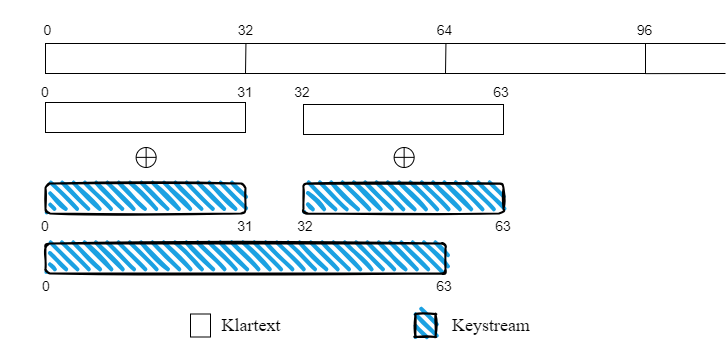
\includegraphics[width=0.9\textwidth]{pictures/avx_updated.png} 
  \caption{Parallele Verarbeitung von 32 Bytes mit AVX } 
  \label{fig:my_label}
\end{figure}


\subsubsection{Rückwärtskompatibilität}
Für Maschinen, die den AVX-Befehlssatz nicht unterstützen, wurde die Rückwärtskompatibilität sichergestellt, indem stattdessen Befehle aus dem SSE-Befehlssatz verwendet wurden. Dazu wurde zur Laufzeit geprüft, ob der AVX-Befehlssatz von der Maschine unterstützt wird, und ein anderer Codepfad falls nicht erstellt, der SSE-Intrinsics verwendet. Dies bedeutete auch, dass anstelle der Verarbeitung von zwei Sätzen von 256 Bits nun vier Sätze von jeweils 128 Bits nacheinander verarbeitet werden sollten.


\subsubsection{Alignment}
Eine weitere Optimierung, die im Programm vorgenommen wurde, war die Sicherstellung der Speicherausrichtung bei der Speicherallokation für den Klartext und den verschlüsselten Text. Das Alignment für die Eingabe- und Ausgabematrix, die als Parameter an die Kernfunktion übergeben werden, wurde ebenfalls sichergestellt, da auf diese ebenfalls häufig zugegriffen wird. Der Gedanke dahinter ist, dem Prozessor die geringste Anzahl von Speicherzugriffen zu ermöglichen und damit ein wesentlich schnelleres Programm zu erhalten. Es wurde eine Speicherausrichtung an einer Grenze von 32 Bytes implementiert, da die verwendeten AVX-Instruktionen eine Speicherausrichtung an einer Grenze von 32 Bytes erfordern. Die verwendeten SSE-Befehle erfordern hingegen eine Ausrichtung an einer Grenze von 16 Byte, was jedoch automatisch abgedeckt wird, wenn der Speicher bereits an einer 32-Byte-Grenze ausgerichtet ist, da 32 durch 16 teilbar ist.
%performance gain by using aligned instructions referenced here
\subsubsection{Optimierungen in der Kernfunktion}
Die Verwendung von Intrinsics in der Verschlüsselungsfunktion hatte zu erheblichen Leistungssteigerungen geführt, die später in der Leistungsanalyse eingehend untersucht werden. Nun aber wurde die Kernfunktion scheinbar der Flaschenhals für das gesamte Programm. Die Transponierungsfunktion und die Bit-Rotationsfunktion waren einige der teuren Operationen, die in der Kernfunktion aufgerufen wurden und die weiter optimiert werden konnten 

Da C keinen Bit-Rotationsoperator bereitstellt, wurde eine Funktion in C implementiert, die dieselbe Operation durchführt. Diese Funktion enthielt zwei Speicherzugriffe, zwei Bit-Shift-Operationen, eine Subtraktion und eine Bit-oder-Operation. Um dies zu optimieren, wurde hier stattdessen eine Funktion in Assembler verwendet, die den ROL-Befehl nutzt. Um die vom Compiler durchgeführten Optimierungen weiter auszunutzen, wurde diese Bitrotationsfunktion \verb{ rotate_bits_asm{ mit dem Attribut\verb{ hot{ deklariert, um den Compiler wissen zu lassen, dass diese Funktion häufig aufgerufen wird, damit der Compiler aggressive Optimierungen vornehmen könnte.

Eine weitere Operation, die die Kernfunktion verlangsamte, war die Transponierungsfunktion. Die Gesamtzahl der Iterationen für eine einzelne Kernmatrix beträgt 20. Am Ende jeder Iteration musste die 4x4-Matrix transponiert werden, bevor die nächste Reihe von Operationen ausgeführt werden konnte. Diese Funktion wurde jedoch dadurch überflüssig, dass die nächste Reihe von Operationen einfach auf dem bestehenden, nicht transponierten Array in der transponierten Ordnung ausgeführt wurde. Zum Beispiel wird statt auf die Elemente 4 und 9 in der transponierten Matrix auf die Elemente 1 und 6 in der nicht transponierten Matrix zugegriffen.
Durch das Überspringen des Transponierungsschritts wird unnötiger Rechenaufwand vermieden, und die Operationen können effizienter an der bestehenden, nicht transponierten Matrix durchgeführt werden.

\begin{figure}[h] 
  \centering 
  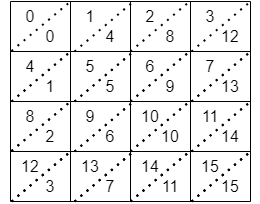
\includegraphics[width=0.9\textwidth]{pictures/transpose.png} 
  \caption{Transponierte und nicht transponierte 4x4 Matrix } 
  \label{fig:my_label4}
\end{figure}

\subsubsection{Mögliche weitere Optimierungen}
Selbst mit all diesen Optimierungen war die Kernfunktion immer noch ein Flaschenhals in Bezug auf die Leistung. Auch wenn es ein erkennbares Muster zwischen den Instruktionen innerhalb der Iterationen gab, waren die Datensätze nicht nur klein, sondern es bestanden auch komplexe Datenabhängigkeiten zwischen den Operationen und zwischen nachfolgenden Iterationen. Daher stellt die Anwendung von SIMD auf die Kernfunktion eine Herausforderung dar. Selbst wenn die Operationen parallelisiert würden, wäre der Leistungsaufwand, der sich aus dem Einzelzugriff auf die unregelmäßig getrennten Arrayelemente und der Speicherung der Elemente an verschiedenen Arraypositionen nach der Verarbeitung ergeben würde, beträchtlich, und in Anbetracht der Anwendung über 20 Iterationen waren wir wirklich unsicher, ob wir überhaupt einen Leistungsgewinn erzielen könnten.

Eine andere Idee bestand darin, die Instruktionen in einer Weise neu anzuordnen, die die Cache-Effizienz erhöht, wobei jedoch die Datenabhängigkeiten berücksichtigt werden. 



\section{Korrektheit}
Wir bevorzugen Korrektheit gegenüber Genauigkeit, da es sich bei unserem Programm, einem symmetrischen Verschlüsselungsalgorithmus, um ein "Hit or Miss" handelt. Das bedeutet, dass wir entweder das Programm korrekt implementiert haben, den korrekten verschlüsselten Text erzeugen und die Originaldatei zurückgeben können, wenn wir den verschlüsselten Text ausführen. Wir beschäftigen uns nicht mit einem Genauigkeitsvergleich.

Die Gewährleistung der Korrektheit eines symmetrischen Verschlüsselungsalgorithmus kann eine Herausforderung darstellen, da der Algorithmus deterministisch ist und immer die entschlüsselte Nachricht zurückgibt, wenn derselbe Schlüsselstrom verwendet wird, selbst wenn die Erzeugung des Schlüsselstroms nicht genau wie beim salsa20/20-Algorithmus durchgeführt wurde. In diesem Abschnitt möchten wir erklären, wie wir die Korrektheit unseres Programms gewährlesiten. Um sicherzustellen, dass unser Programm korrekt ist, haben wir zwei Korrektheitsprüfungen durchgeführt. Diese werden mit dem Option -d als Korrektheitscheck durchgeführt. 

V0 steht für unsere Hauptimplementierung mit vektorisiertem SIMD-Ansatz (Single Instruction Multiple Data) für das ARX-Schema und V1 als die Standard- oder naive Implementierungsversion. Zunächst stellen wir sicher, dass sowohl V0 als auch V1 denselben Chiffrierstrom erzeugen. Dies geschieht mit der Option -d, indem wir dieselbe Eingabedatei mit beiden Implementierungen ausführen. Derselbe Schlüssel und dieselbe Nonce wird dafür verwendet, um die Matrix zu erzeugen. Danach werden die beiden entschlusselten Text miteinander verglichen. Das Programm führt einfach eine XOR-Operation zwischen dem Eingabetext und der Keystrom-Block durch. Wenn beide Implementierungen den gleichen verschlüsselten Text erzeugen, können wir daraus schließen, dass sie auch die gleiche Stromchiffre erzeugt haben. 

Zweitens wollen wir sicherstellen, dass der symmetrische Teil unseres Algorithmus wie erwartet funktioniert. Dazu führen wir das Programm zunächst mit einem beliebigen Schlüssel und einer beliebigen Nonce auf einer beliebigen Eingabedatei aus und schreiben die Ausgabe in die Datei output.txt. Der nächste Schritt besteht darin, genau denselben Schlüssel und dieselbe Nonce zu nehmen und sie dann zusammen mit output.txt als Programmeingabe zu verwenden. Auf diese Weise können wir leicht feststellen, dass die resultierende Datei mit der Originaldatei identisch ist. 

\section{Performanzanalyse}
In diesem Abschnitt möchten wir den Vergleich zwischen unseren beiden Implementierungsversionen genauer betrachten. Die Messung wurde auf einem Rechner mit 3.10 GHz, 10-Core Intel(R) Xeon(R) E5-2687W v3 CPU durchgeführt. Das Programm wurde mit Visual Studio Code ausgeführt.

Wir haben zwei Messungen gemacht, nämlich bei der Core-Funktion und dann das gesamte Programm. Im Tabelle 1 steht die durchschnittliche Zeit für \verb {salsa20_core{ Funktion (mit ASM Implementierung für die Bit-Operation) und \verb{salsa20_core_v1{ in Mikrosekunde.

%%%% TODO %%%%
\begin{table}[h]
\centering
\begin{tabular}{|c|c|c|}
\hline
& \verb{salsa20_core{ & \verb{salsa20_core_v1{ \\
\hline
Average time & 2.5097$\upmu$s & 4.0147$\upmu$s \\
\hline
\end{tabular}
\caption{Zeitmessung der core Funktion}
\end{table}

Aus den Daten lässt sich eine Beschleunigung von rund 37,49\% ableiten. Dies ist darauf zurückzuführen, dass wir ASM-Anweisungen für unsere Operationen verwenden.Da der Assembler-Code keinen Compiler durchlaufen muss, benötigt er auch weniger CPU-Zeit. Mit ASM entsteht auch weniger Overhead von Funktionsaufruf, weil wir bei normalen Funktionsaufruf die Registerwerte speichern müssen und die Return-Adresse auf dem Stack mit PUSH und POP bearbeiten. Außerdem greifen wir auch auf die transponierten Elemente zu, ohne eine Funktion aufzurufen, die die Elemente im Speicher mit ihren transponierten Elementen überschreibt. Dies führt ebenfalls zu einer Leistungssteigerung.

Jetzt bertrachten wir die Messung von unserem gesamten Programm. Die Laufzeit beider Implementierungen wird mit der Funktion \verb{clock(){ in C gemessen, die zweimal aufgerufen wird: einmal vor der Hauptfunktion und einmal nach deren Beendigung. Die Differenz zwischen diesen beiden Werten wird dann durch \verb{CLOCKS_PER_SEC{ geteilt, um die tatsächliche Zeit in Sekunden zu erhalten. Wir wählen die Funktion \verb{clock(){ gegenüber der Funktion \verb{CLOCK_MONOTONIC{ in \verb{clock_getTime(){ aus zwei Gründen: 
\begin{enumerate}
    \item \verb{clock(){ ist Teil der C-Standardbibliothek \cite{ClockManPage}, während \verb{clock_getTime(){ eine POSIX-Funktion ist, die nur für Unix-like Systeme verfügbar ist.
    \item  \verb{clock(){ misst die tatsächlich verbrauchte CPU-Zeit, während \verb{clock_getTime(){ die sogenannte wall-clock Zeit \cite{ClockGetTimeManPage}. 
\end{enumerate}

Da wir nur an der Messung und dem Vergleich der Leistung unseres Codes interessiert sind, haben wir uns für die Funktion \verb{clock(){ entschieden. Bei der Messung haben wir die Option -B 1000 gesetzt, um das Programm 1000 mal wiederzuholen und die durschnittliche Zeit zu berechnen. Den Vergleich ist auf Abbildung 3 gezeigt. 


\begin{figure}[h] 
  \centering 
  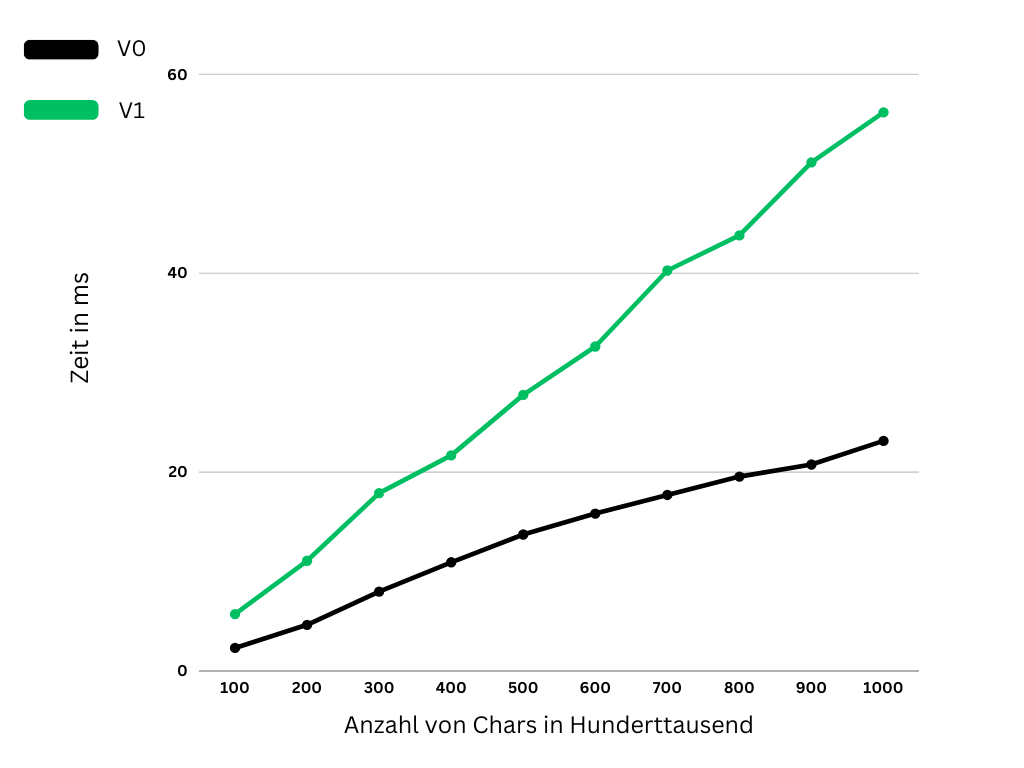
\includegraphics[width=0.90\textwidth]{pictures/benchmark10.png} 
  \caption{Benchmark Graph} 
  \label{fig:my_label2}
\end{figure}

Aus den Daten, können wir zwei Dinge schließen: Erstens skalieren unsere beiden Implementierungen linear mit der Größe der Eingabedatei. Dies ist das erwartete Verhalten für den Salsa20-Verschlüsselungsalgorithmus, da wir nur grundlegende Operationen an den Daten durchführen. Zweitens können wir sehen, dass die Benutzung von SIMD und ASM in unser Programm eine durchschnittliche Beschleunigung von 53,76\% bringt. Durch die vektorisierte Datenverarbeitung mit SIMD können wir 256 Bits auf einmal berechnen, was bei der naive Implementierung nicht der Fall ist. Dadurch entsteht die Leistungssteigerung.


\section{Zusammenfassung und Ausblick}
Zusammenfassend wurde die Funktionsweise der von Daniel J. Bernstein erfundenen Stromchiffre Salsa20/20 in dieser Ausarbeitung vorgestellt. Wir haben zwei Ansätze implementiert und konnten daraus feststellen, dass durch Verwendung von SIMD und Assembly eine Leistungssteigerung gewonnen werden kann. Um zu zeigen, dass die beiden Implementierungen dasselbe Ergebnis liefern, wurden die Ergebnisse der Implementierungen verglichen.

Als Ausblick glauben wir, dass die Kernfunktion durch die Verwendung von Intrinsics und die Erhöhung der Cache-Effizienz weiter optimiert werden könnte. Aufgrund der komplexen Datenabhängigkeiten, die durch die Anordnung der Instruktionen entstehen, fanden wir es sehr schwierig, die Cache-Misses zu reduzieren und die Programmleistung zu erhöhen. Diese Ansätze sollten jedoch getestet und analysiert werden, um zu sehen, ob sie tatsächlich zu einem Leistungsgewinn führen.

% TODO: Fuegen Sie Ihre Quellen der Datei Ausarbeitung.bib hinzu
% Referenzieren Sie diese dann mit \cite{}.
% Beispiel: CR2 ist ein Register der x86-Architektur~\cite{intel2017man}.
\bibliographystyle{plain}
\bibliography{Ausarbeitung}{}

\end{document}
